\entry{2026-10-20}{Burgers 2D/3D campaign: final compilation}

All ten lanes of the campaign (\path{reports/2026-10-17-full-experiment-plan/}) are finished and compiled by \texttt{final/make\_final.py} into \path{final/report.md} (every number traced in \texttt{PROVENANCE.json}; Codex final audit round 12 CLEAN). Total compute 168.8 GPU-h. Development/validation cohorts only; sealed and reserved-OOD cohorts unopened; E0-conditional errors.

\begin{itemize}
\item \textbf{The advisor's question.} Solve cost does not depend on the mesh (2D and 3D, both readings of $k$, across retraining seeds and GPU types); accuracy does not depend on the mesh; accuracy improves with bank width up to $r=384$ (not to 512); kernel cost does not follow the registered operation-count exponents.
\item \textbf{Competition.} K2 fires in 2D and 3D: a coarse spectral solver matches the ROM's accuracy faster. H-base fails: a tuned POD + ECSW/Q-DEIM model dominates our qualified 2D configurations at $256^2$ and $1024^2$.
\item \textbf{Robustness and generality.} Not qualified on steeper fronts than in training (the bank cannot represent them); degrades in the stiff corner of its own range. Mesh-independence and the $r$ dial survive retraining; the quadrature rule must be selected per bank.
\item \textbf{What the paper can claim:} mesh-independent cost, mesh-free (continuum) evaluation and memory; speed and accuracy advantages over standard alternatives are not supported for viscous Burgers on the box.
\end{itemize}
\begin{center}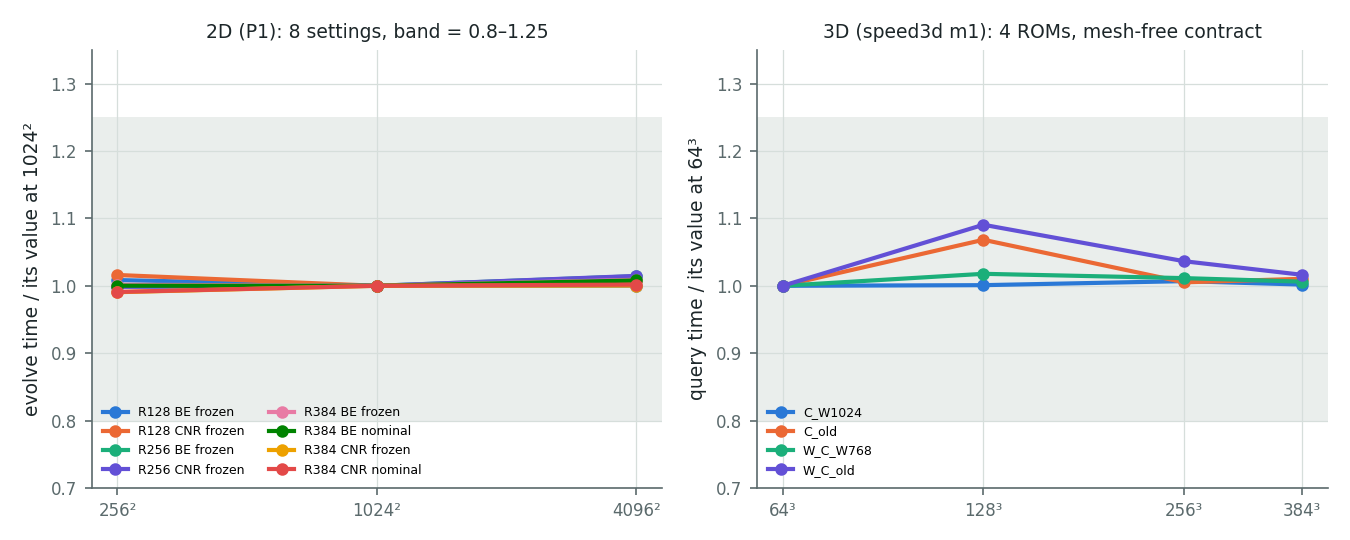
\includegraphics[width=0.48\linewidth]{figs/final_cost_vs_mesh.png}\hfill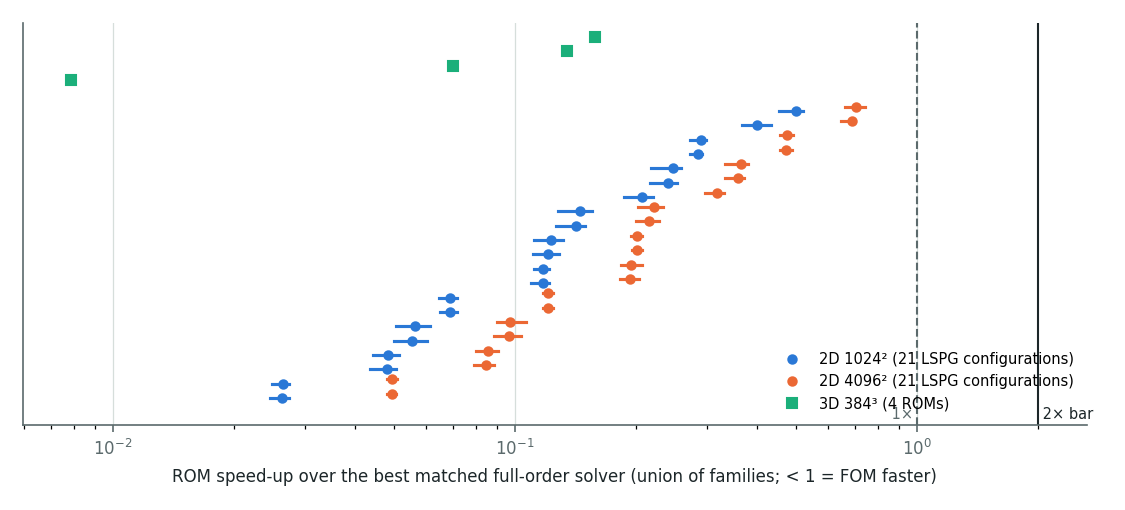
\includegraphics[width=0.48\linewidth]{figs/final_union_speedup.png}\end{center}
Branches of all ten lanes await the user's merge decision.
